
\renewcommand{\arraystretch}{1.5} % Default value: 1

%%% Write here
%%%%%%%%%%%%%%%%%%%%%%%%%%%%%%%%%%%%%
\section{Introduction}
The Faraday effect, also known as Faraday rotation, is a magneto-optic phenomenon that demonstrates the fundamental interaction between light and a magnetic field. Discovered by Michael Faraday, this effect reveals that isotropic media become optically active when a magnetic field is applied parallel to the propagation direction of the light. This pivotal observation served as one of the earliest indications of the deep, underlying connection between optics and electromagnetism. Specifically, introducing a magnetic field in the direction of a light beam's propagation through a transparent medium induces a phenomenon known as circular birefringence.

As linearly polarized light travels through the optical medium under these conditions, its plane of polarization undergoes a measurable rotation. The angle of this rotation is a linear function of both the mean magnetic flux density and the length of the optical medium. The factor of proportionality governing this relationship is known as Verdet's constant. This specific experiment focuses on measuring and interpreting this magnetically induced circular birefringence.
%%%%%%%%%%%%%%%%%%%%%%%%%%%%%%%%%%%%%
\section{Objective}
The objective of this experiment is to measure and interpret the magnetically induced circular birefringence known as the Faraday effect.
%%%%%%%%%%%%%%%%%%%%%%%%%%%%%%%%%%%%%
\section{Equipment Required}
Here is the list of required equipment for the Faraday effect setup:
\begin{enumerate}
    \item \textbf{Light Source:} Red diode lasers with wavelengths of 650 nm, secured on a laser mount.
    \item \textbf{Polarizing Filters:} A polarizer rotator to polarize the incident light and a precision polarizer mount acting as an analyzer.
    \item \textbf{Magnetic Field Generator:} An electromagnet formed by a long solenoid with 2508 turns of wire, connected to a magnet power supply. Number of turns per unit length is 167.2 /cm.
    \item \textbf{Optical Medium:} A transparent flint glass rod, which serves as the sample placed inside the solenoid.
    \item \textbf{Detection System:} A photodiode detector used to measure the intensity of the light beam after it passes through the analyzer.
    \item \textbf{Mounting Apparatus:} A linear optical rail equipped with translating mounts. This track facilitates the secure attachment and precise spatial alignment of all optical components, ensuring the beam remains centered through the sample and upon the active area of the detector.
\end{enumerate}

\begin{figure}[H]
    \centering
    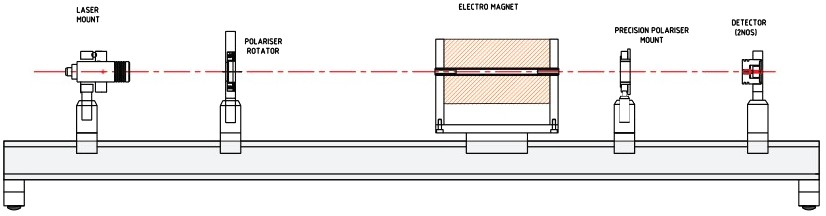
\includegraphics[width = 0.9\textwidth]{Image/setup2.jpg}
    \caption{Schematic of Faraday setup}
    \label{fig:setup2}
\end{figure}
%%%%%%%%%%%%%%%%%%%%%%%%%%%%%%%%%%%%%
\section{Theory}
%%%%%%%%%%%%%%%%%%%%%%%%%%%%%%%%%%%%%
\section{Procedure}
We have followed the following procedure to do this experiment:
\begin{enumerate}
    \item First we placed the laser, P1 (polarizer), Faraday tube or that electro magnet on the optical rail (see \cref{fig:setup1}).
    \item Then we did the alignment of the laser. To do so we first measured the height of the laser near the source and near the detector and matched it. We assured that the beam was completely passing through the tube (Electro magnet).
    \item Then we changed the angle of the P1 to have maximum intensity in the detector. Note that we kept the current zero at this configuration and we did not place the P2 at the rail. 
    \item Next we put the P2 (polarizer) and made the configuration such that the intensity is minimum at the detector.
    \item In this setup we did this experiment which had two part. In the first part we measured the variation of the angle of the rotation due to the magnetic effect and in the later part we measured the variation of the intensity over the current (i.e. magnetic field strength).
\end{enumerate}

\begin{figure}[H]
    \centering
    \includegraphics[width = 0.8\textwidth]{Image/setup_img.JPG}
    \caption{Setup for Faraday Effect}
    \label{fig:setup1}
\end{figure}


%%%%%%%%%%%%%%%%%%%%%%%%%%%%%%%%%%%%%
\section{Data analysis and calculation} 

\begin{longtable}{|c|c|c|c|c|}


\caption{Rotation of angle due to the Faraday-Magnetic effect} \\
\toprule

Current & Magnetic field & Theta in P2(Degrees) & Angle(Diff) (min) & Verdet constant \\

\midrule
\endfirsthead

\multicolumn{5}{c}%
{{\bfseries Table \thetable\ -- continued from previous page}} \\
\toprule
Current & Magnetic field & Theta in P2(Degrees) & Angle(Diff) (min) & Verdet constant \\
\midrule
\endhead

\midrule
\multicolumn{5}{|r|}{Continued on next page} \\
\bottomrule
\endfoot

\bottomrule
\endlastfoot

% data
0       & 0              & 112                  & 0                 &    $\dots$      \\
0.4     & 210.1097167    & 112.4                & 24                & 0.011422604     \\
0.8     & 420.2194333    & 113.2                & 72                & 0.017133905     \\
1.22    & 640.8346358    & 113.9                & 114               & 0.017789301     \\
1.6     & 840.4388667    & 114.5                & 150               & 0.017847818     \\
2.02    & 1061.054069    & 115.2                & 192               & 0.018095214     \\
2.4     & 1260.6583      & 116                  & 240               & 0.019037673     \\
2.79    & 1465.515274    & 116.9                & 294               & 0.020061203     \\
3.22    & 1691.383219    & 117.2                & 312               & 0.018446441     \\
3.59    & 1885.734707    & 117.8                & 348               & 0.018454346     \\
4.02    & 2111.602653    & 118.7                & 402               & 0.019037673     \\
4.29    & 2253.426711    & 119.4                & 444               & 0.019703326   
\end{longtable}

\begin{figure}[H]
    \centering
    
\includegraphics[width = 0.8\textwidth]{../data analysis/Plot1.pdf}
    \caption{Variation of optical rotation angle over applied magnetic field}
    \label{fig:plot1}
\end{figure}

\begin{longtable}{|c|c|c|}

\caption{Table for variation of intensity over current variation} \\
\toprule

Current & Magnetic field & Intensity ($\mu A$) \\

\midrule
\endfirsthead

\multicolumn{3}{c}%
{{\bfseries Table \thetable\ -- continued from previous page}} \\
\toprule
Current & Magnetic field & Intensity ($\mu A$) \\
\midrule
\endhead

\midrule
\multicolumn{3}{|r|}{Continued on next page} \\
\bottomrule
\endfoot

\bottomrule
\endlastfoot
%
0       & 0              & 0.8            \\
0.4     & 210.1097167    & 1.3            \\
0.84    & 441.230405     & 2.5            \\
1.12    & 588.3072067    & 4.1            \\
1.63    & 856.1970954    & 6.9            \\
2.05    & 1076.812298    & 9.8            \\
2.43    & 1276.416529    & 12.8           \\
2.83    & 1486.526245    & 16.2           \\
3.16    & 1659.866762    & 20.3           \\
3.6     & 1890.98745     & 24.5           \\
3.99    & 2095.844424    & 28.4  
\end{longtable}

\begin{figure}[H]
    \centering
    
\includegraphics[width = 0.8\textwidth]{../data analysis/Plot2.pdf}
    \caption{Variation of Intensity over current}
    \label{fig:plot2}
\end{figure}
%%%%%%%%%%%%%%%%%%%%%%%%%%%%%%%%%%%%%
\section{Sources of Error}

\subsection{Thermal and Environmental Effects}
\begin{itemize}
    \item \textbf{Sample Heating:} The resistive heating of the electromagnet coil can transfer heat to the flint glass sample. This temperature increase can alter the Verdet constant of the glass and produce convection currents that locally vary the refractive index, introducing unwanted intensity changes.
    \item \textbf{Laser Intensity Drift:} Semiconductor diode lasers often exhibit slow temporal variations in output intensity, particularly before the laser reaches thermal equilibrium. If the laser is not allowed sufficient warm-up time, this drift can be mischaracterized as a change in transmitted intensity due to polarization rotation.
\end{itemize}

\subsection{Instrumental and Alignment Limitations}
\begin{itemize}
    \item \textbf{Detector Non-linearity and Spatial Sensitivity:} The photodiode signal may not respond perfectly linearly to incident light intensity. Furthermore, if the laser beam is not strictly centered on the active area of the photodiode, any slight beam deflection caused by rotating the optical components can cause spurious intensity readings.
    \item \textbf{Magnetic Field Non-uniformity:} The standard theoretical formula $\varphi = VHL$ assumes a perfectly uniform magnetic field $H$ across the entire length of the optical medium. In reality, the field lines begin to diverge near the ends of the solenoid, meaning the magnetic field is not perfectly constant across the entire length of the glass rod.
\end{itemize}

\subsection{Observational Uncertainty}
\begin{itemize}
    \item \textbf{Parallax Error in Angular Measurement:} The physical design of the setup, specifically the proximity of the electromagnet's cylindrical housing to the analyzing polarizer, restricts the observer's direct line of sight to the graduated scale. This obstruction forces the experimenter to read the angle from an oblique viewing position, introducing a parallax error that reduces the precision of the rotational measurements.
    \item \textbf{Resolution of the Null Point:} Accurately determining the exact angle of minimum transmitted intensity (the "darkness" point) is limited by the mechanical resolution (least count) of the precision polarizer mount. Additionally, at near-zero intensity, the signal-to-noise ratio of the photodiode drops, making the exact minimum difficult to pinpoint precisely.
    \item \textbf{Backlash Error:} Mechanical play or backlash in the rotational mount of the analyzing polarizer can introduce discrepancies if the minimum intensity angle is approached from different directions (clockwise vs. counter-clockwise). Though while taking the reading we maintain single convention (clockwise) to make the P2 for minimum intensity.
\end{itemize}
%%%%%%%%%%%%%%%%%%%%%%%%%%%%%%%%%%%%%
\section{Conclusion}
%%%%%%%%%%%%%%%%%%%%%%%%%%%%%%%%%%%%%